\section{Historical Introduction to Quantum Mechanics}

\subsection{Particles and Waves in Classical Mechanics}

Classical mechanics is based on two distinct concepts: particles and waves.

Particles are:
\begin{itemize}
    \item point-like objects,
    \item described using a location vector \(\vb{x}\pqty{t}\),
    \item obeying Newton's 2nd law of motion (second-order ODE) \(m \ddot{\vb{x}}\pqty{t} = \vb{F}\pqty{\vb{x}\pqty{t}, \dot{\vb{x}}\pqty{t}}\),
    \item with initial conditions \(\vb{x}\pqty{t_0}\) and \(\dot{\vb{x}}\pqty{t_0}\) gives the solution to all times,
    \item and there is no interference between two particles.
\end{itemize}

Waves are 
\begin{itemize}
    \item spread-out objects,
    \item described using a function \(f\pqty{\vb{x}, t}\) which is periodic in \(t\) or \(\vb{x}\),
    \item obeying the wave equation (second-order PDE) \(\pdv[2]{f\pqty{\vb{x}, t}}{t} - c^2 \laplacian f\pqty{\vb{x}, t} = 0\),
    \item with solutions as superposition of
    \[
        f_{\pm} \pqty{\vb{x}, t} = A \exp\pqty{i \pqty{\pm \vb{k} \vdot \vb{x} - \omega t}}
    \]
    where \(A \in \CC, \vb{k} \in \RR^3\) and \(\omega \in \RR\) are constants,
    \item solutions obey dispersion \(\boxed{\omega = c \abs{\vb{k}}}\) where \(\omega\) is the \emph{angular frequency} which is related to \(\lambda\), the \emph{wavelength}, and the frequency \(\nu\), by
    \[
        \omega = 2\pi \nu = \frac{2\pi c}{\lambda},
    \]
    \item and waves interfere with each other, by constructive or destructive interference.
\end{itemize}

\subsection{Light (Electromagnetic Waves) behaving like a Particle}

\subsubsection{Black-Body Radiation (Non-Examinable)}

\subsubsection{Photoelectric Effect}

\begin{figure}[ht!]
    \centering
    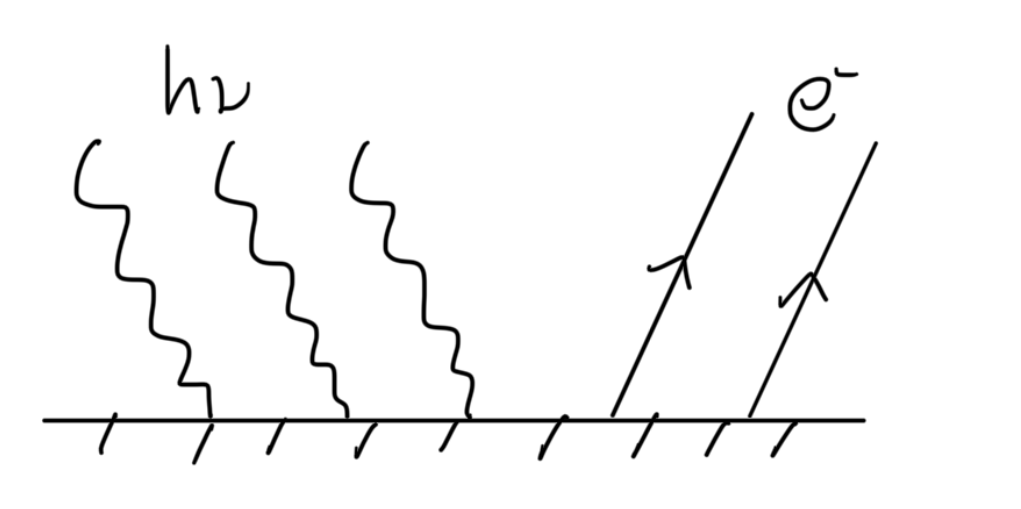
\includegraphics[scale=0.5]{fig/photoelectric-effect.png}
    \caption{The Photoelectric Effect Experiment}
    \label{fig:photoelectric-effect}
\end{figure}

The photoelectric effect, as illustrated in \autoref{fig:photoelectric-effect}, is discovered as follows. We fix the wavelength \(\lambda\) (and hence \(\nu, \omega\) of light) for each beam, aimed towards a piece of metal, and we change the intensity of light \(I = \abs{A}^2\), where \(A\) is the amplitude of the light wave.

A classical expectation is as follows:
\begin{enumerate}[label=(\roman*)]
    \item because incident light has \(E \propto I\), as the intensity increases, once the threshold value (\(I_0\)) is reached, then \Pelectron are emitted.
    \item the emission rate of \Pelectron is proportional to \(I\) (the intensity of light).
\end{enumerate}

However, we observed the following.

\begin{enumerate}
    \item Below a given \(\omega\) (i.e. above a given \(\lambda\)), there is no \Pelectron emitted, no matter how high the intensity is.
    \item The velocity of \Pelectron is dependent on \(\omega\), not \(I\).
    \item Emission rate of \Pelectron is proportional to \(I\).
\end{enumerate}

In 1905, Einstein proposed that light comes in small quanta, which are called \term{photons} \Pphoton, and each quantum of light carries an energy given by
\[
    E = \hbar \omega = h \nu
\]
where \(\hbar = \flatfrac{h}{2\pi}\), and \(h\) is the \term{Planck constant} with value \(h \approx \SI{6.6e-34}{\joule\second}\), and momentum given by
\[
    \vb{p} = \hbar \vb{k}.
\]

Simply by assuming the conservation of energy, this explains this phenomena: in particular, the \term{threshold frequency} is therefore
\[
    E_{\min} = 0 = \hbar \omega_{\min} - \phi
\]
where \(\phi\) is the \term{binding energy} of the electrons. This explains the corresponding observations.
\begin{enumerate}
    \item If we are below \(\omega_{\min} = \flatfrac{\phi}{\hbar}\), no electrons may escape the piece of metal.
    \item The kinetic energy of escaping \Pelectron is given by \(E = \hbar \omega - \phi\) for \(\omega > \omega_{\min}\).
    \item We also understand that the larger the intensity \(I\), the more light quanta we have, and hence the more scattering events with \Pelectron, hence a higher emission rate.
\end{enumerate}

\subsubsection{Compton Scattering (Non-Examinable)}

\subsection{Atomic Spectra}

\begin{figure}[ht!]
    \centering
    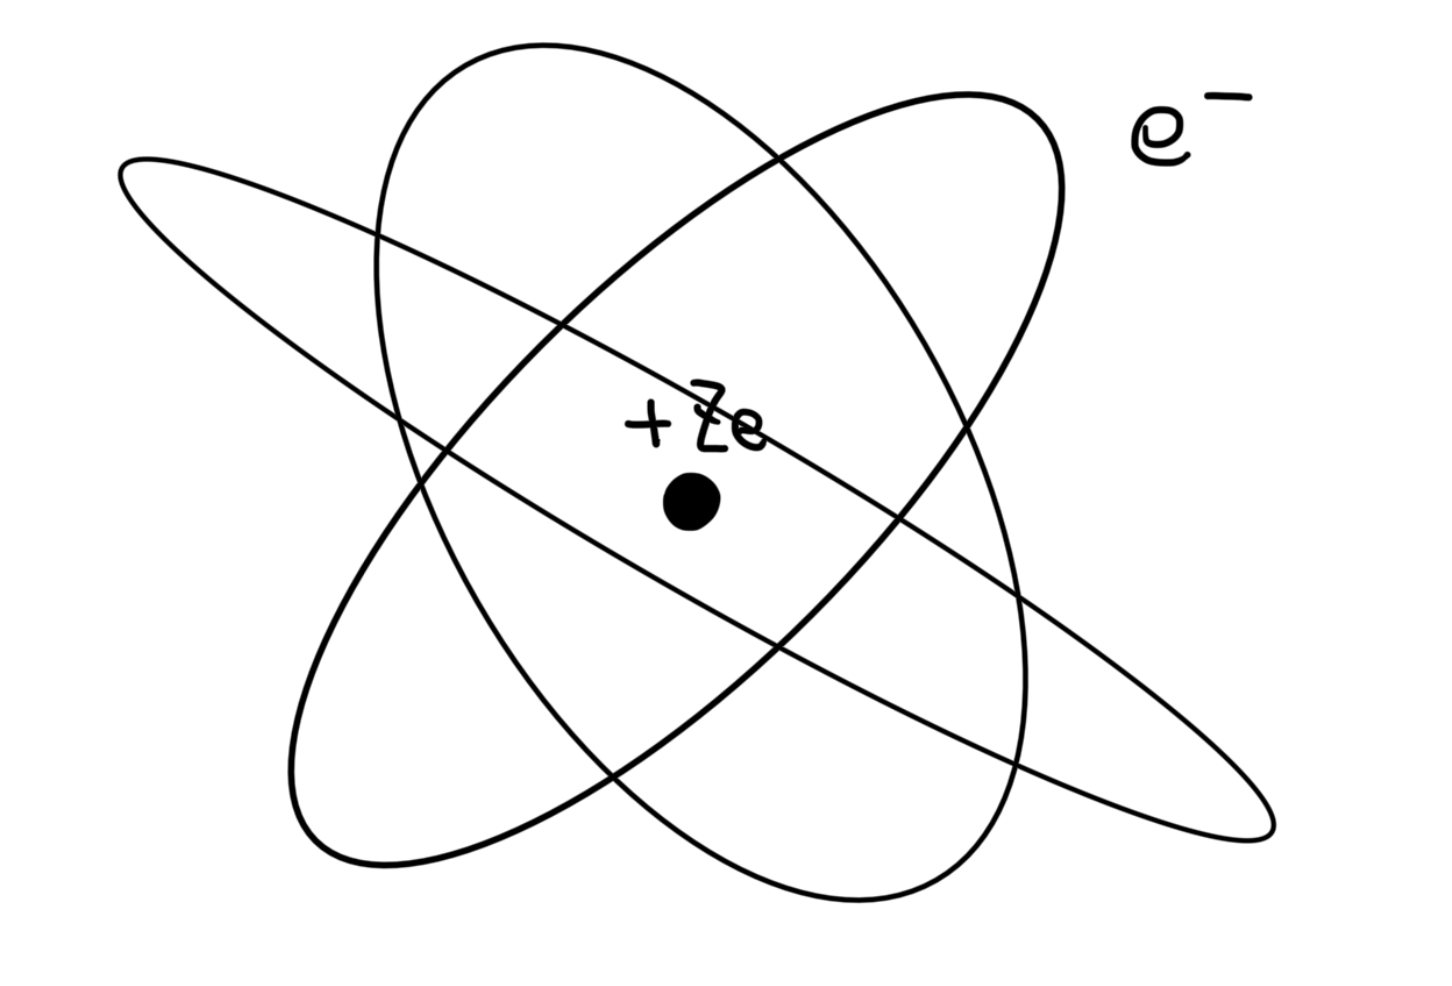
\includegraphics[scale=0.5]{fig/rutherford-model.png}
    \caption{The Rutherford Model of the Atom}
    \label{fig:rutherford-model}
\end{figure}

The Rutherford model (1908), illustrated in \autoref{fig:rutherford-model}, suggests that electrons with charge \(-e\) orbit around a nucleus charged at \(+Ze\). This model cannot hold for three reasons.

\begin{enumerate}[label=(\roman*)]
    \item The \Pelectron on orbits around nucleus would radiate energy.
    \item The \Pelectron would collapse, eventually, onto the nucleus.
    \item Experimentally measured atomic spectra were discrete. In particular, light emitted by atoms when hit by light was described by a set of lines
    \[
        \omega_{mn} = 2 \pi c R_0 \pqty{\frac{1}{n^2} - \frac{1}{m^2}},
    \]
    where \(R_0\) is the \term{Rydberg constant}.
\end{enumerate}

Bohr explained these evidence using a simple postulate, that the orbitals angular momentum may only take discrete values, given by
\[
    L_n = \hbar n, \quad n \in \NN.
\]

This quantisation of \(L\) explains the quantisation of \(r, v\) and \(E\) as follows for a hydrogen atom.

Assuming a circular orbit, we have \(L = m_{\Pe} v r\), and hence \(v = \flatfrac{L}{m_{\Pe} r}\). Putting the postulate in, this leads to
\[
    v_n = \frac{n \hbar}{m_{\Pe} r}.
\]

From the Coulomb force, we have
\[
    \frac{e^2}{4 \pi \epsilon_0} \frac{1}{r^2} = m_{\Pe} \frac{v^2}{r}
\]
and hence
\[
    r_n = \frac{4 \pi \epsilon_0}{m_{\Pe} e^2} n^2 \hbar^2.
\]

In particular, this predicts the minimal radius of electron orbit, the \term{Bohr radius}, given by
\[
    r_1 = \frac{4 \pi \epsilon_0}{m_{\Pe} e^2} \hbar^2.
\]

Furthermore, we have quantised energy, given by
\[
    E_n = \frac{1}{2} m_{\Pe} v_n^2 - \frac{e^2}{4 \pi \epsilon_0} \frac{1}{r_n} = - \frac{e^2}{8 \pi \epsilon_0 r_1} \frac{1}{n^2}.
\]

When an electron drops from a higher level to a lower level, we have
\[
    \hbar \omega_{mn} = E_m - E_n
\]
and hence
\[
    \omega_{mn} = \frac{m_{\Pe} c^2 \alpha^2}{2\hbar}\left(\frac{1}{n^2}-\frac{1}{m^2}\right)
\]
where \(\alpha\) is the (dimensionless) \term{fine structure constant}, given by
\[
    \alpha = \frac{e^2}{4 \pi \epsilon_0 \hbar c} \approx \frac{1}{137},
\]
and we recover \(R_0\) identical to experimental evidence, namely
\[
    R_0 = \frac{m_{\Pe} c \alpha^2}{4\pi \hbar}.
\]

However, we will return to this in a future chapter, where we solve the Schr\"{o}dinger equation, to conclude that in fact Bohr was not correct with this model.

\subsection{Particles Interfering with Each Other}

\subsubsection{De Broglie Principle}

\subsubsection{Diffraction of Electrons (\Pelectron)}